\documentclass[11pt]{article}

\usepackage{graphicx}
\usepackage[colorlinks=true, linkcolor=blue]{hyperref}
\usepackage[italian]{babel}
%\selectlanguage{italian}
\usepackage[utf8]{inputenc}
\usepackage[svgnames]{xcolor}
\usepackage{amsmath}
\usepackage{enumitem}
\usepackage{multicol}
\usepackage{enumitem}
\usepackage{amssymb}

\usepackage{listings}
\usepackage{afterpage}

\usepackage{float}
\restylefloat{table}

\pagestyle{plain}

\definecolor{dkgreen}{rgb}{0,0.6,0}
\definecolor{gray}{rgb}{0.5,0.5,0.5}
\definecolor{mauve}{rgb}{0.58,0,0.82}

%\lstset{language=Python,
%    basicstyle=\small\ttfamily,
%   stringstyle=\color{DarkGreen},
%    otherkeywords={0,1,2,3,4,5,6,7,8,9},
%    morekeywords={TRUE,FALSE},
%    deletekeywords={data,frame,length,as,character},
%    keywordstyle=\color{blue},
%    commentstyle=\color{DarkGreen},
%}

\lstset{frame=tb,
language=R,
aboveskip=3mm,
belowskip=3mm,
showstringspaces=false,
columns=flexible,
numbers=none,
keywordstyle=\color{blue},
numberstyle=\tiny\color{gray},
commentstyle=\color{dkgreen},
stringstyle=\color{mauve},
breaklines=true,
breakatwhitespace=true,
tabsize=3
}


\textheight=21cm
\textwidth=17cm
%\topmargin=-1cm
\oddsidemargin=0cm
\parindent=0mm
\pagestyle{plain}

\usepackage{color}
\usepackage{ragged2e}

\global\let\date\relax
\newcounter{unomenos}
\setcounter{unomenos}{\number\year}
\addtocounter{unomenos}{-1}
\stepcounter{unomenos}
\gdef\@date{ Course \arabic{unomenos}/ 2019}

\begin{document}


\begin{titlepage}

\begin{center}
\vspace*{-1in}
\begin{figure}[htb]
\begin{center}

\includegraphics[width=5cm]{Resources/BicoccaLogo.png}
%\hspace{\fill} %Space between images
%\includegraphics[width=3cm]{sea-vision-official-logo.png}
\end{center}
\end{figure}
UNIVERSITÀ DEGLI STUDI MILANO - BICOCCA \\
\vspace*{0.4in}
\begin{large}
Esame Sistemi Complessi: Modelli e simulazione\\
\end{large}
\vspace*{0.2in}
\begin{Large}
\textbf{Progetto STN} \\
\vspace*{0.15in}
Spreading Tweet News \\
\end{Large}
\vspace*{0.3in}

\vspace*{0.3in}
\rule{80mm}{0.1mm}\\
\vspace*{0.1in}
\begin{large}

Andrea Guzzo - 761818\\
Manuel Zanaboni 816105\\
Vittorio Maggio - 817034\\
Lidia Alecci - 852501


\end{large}
%\includegraphics[width=8cm]{yudoo-image.jpg}
\end{center}
\end{titlepage}

\newcommand{\CC}{C\nolinebreak\hspace{-.05em}\raisebox{.4ex}{\tiny\bf +}\nolinebreak\hspace{-.10em}\raisebox{.4ex}{\tiny\bf +}}
\def\CC{{C\nolinebreak[4]\hspace{-.05em}\raisebox{.4ex}{\tiny\bf ++}}}

\tableofcontents

\newpage

<<<<<<< HEAD
\section{Abstract}

=======
\section{Sommario}
>>>>>>> b895bdc6c2402b095af0f874fcbed27bd2c9b4aa
Una persona passa mediamente 5 anni e 4 mesi della propria vita sui social network, secondo uno studio condotto dall'agenzia di marketing americana Mediakix \cite{mediakix}. Sui social network ci informiamo e discutiamo di tutto ormai, eppure non è sempre un'idea saggia credere a tutto quello che si legge su internet, alcune notizie sono infatti pilotate per raggiungere in minor tempo più persone possibili.
Tale obiettivo è raggiunto impiegando i bot. Quest’ultimi, come qualunque cosa, possono essere sfruttati per motivi nobili (informare di fatti reali che necessitano di raggiungere la popolazione il più in fretta possibile) o per diffondere fake news.
In tale documento verrà discusso la posizione migliore dei bot all’interno di una rete per ottimizzare il numero di persone raggiunte e il tempo impiegato per effettuare la diffusione.

\section{Introduzione}

Oggigiorno i social network rivestono un ruolo chiave nella vita di tutti i giorni, essi infatti influenzano tutti gli aspetti della nostra vita: dal marketing allo shopping, passando per le interazioni con le celebrità ed aziende fino a sostituire, in molte occasioni, le fonti di informazioni primarie come quotidiani o notiziari.

Un report del 2018 effettuato dal Pew Internet research center \cite{ReportPewInternetResearch2018} ha verificato che della popolazione italiana il 64\% usa i social media per informarsi su fatti di cronaca e l’81\% lo usa per informarsi e ricercare pareri su servizi o brand.

Tuttavia, soprattutto negli ultimi anni i social hanno rivestito un ruolo chiave anche nel mondo politico, sia a livello di opinioni politiche che di possibilità di influenzamento del voto degli elettori; ci sono numerosi studi che hanno indagato tali fenomeni.

"Activism in the social media age" \cite{ActivismSocialMedia} ha preso in esame il 53\% della popolazione americana che nell'arco di un anno ha utilizzato i social per ragioni politiche o sociali. Inoltre, da altri sondaggi è emerso che il 69\% della popolazione pensa che i social siano importanti per informare i politici dei problemi che i cittadini si trovano ad affrontare; e il 58\% ritiene che i social media influenzano le decisioni politiche.

Su quest'ultimo punto un’altra importante ricerca "Automating power: Social bot interference in global politics" \cite{AutomaticPower} scende più nello specifico indagando come i Bot sono stati importanti nel veicolare pensieri politici e quindi quanto sono potenzialmente necessari e utili per influenzare le masse. Tale ricerca prende in esame le elezioni di vari paesi e in vari anni, e ,sulla base di altre ricerche effettuate nel corso degli anni, definisce a quale scopo sono stati impiegati i political bot e da chi probabilmente sono stati attivati (se dallo stato stesso o da aziende esterne).

Lo studio effettuato, e le cui specifiche sono descritte nel presente documento, ha l’obiettivo di quantificare l’importanza di selezionare, all’interno di una determinata rete, gli utenti che sono nella posizione migliore di influenzare le masse e che quindi trasformandoli in bot permettono di massimizzare la propagazione di una determinata notizia o pensiero.


\section{Richiami alla teoria}

In questo capitolo verranno descritti alcuni concetti teorici necessari alla comprensione del progetto e che sono stati utilizzati per modellare il problema.
È importante sottolineare come la ricerca scientifica e la progettazione multi-agente su progetti in ambito Social Network Analysis sia relativamente scarsa in quanto esistono differenti punti di vista per affrontare e modellare questo tipo di problemi. Molti lavori in ambito accademico studiano la situazione attraverso considerazioni teoriche sull'analisi a posteriori delle reti sociali, risultando in moltissime metriche e parametri che spesso si dimostrano essere discordanti.

\subsection{Grafo}

Un grafo è una struttura relazionale formata da un numero finito di $V$ di vertici (o nodi) e un numero finito $E$ di segmenti (archi o spigoli) che collegano tra di loro uno o più nodi.
Una definizione più formale è la seguente: “Un grafo è una relazione n-aria su un insieme finito S definita dai sottoinsiemi di $S$ con n elementi che soddisfano una proprietà $P(1,...,n)$”.
Con ordine del grafo viene inteso il numero di nodi esistenti, mentre gli archi di un grafo sono definiti appunto da una relazione (ad esempio binaria) e i nodi che la compongono sono detti estremi dell'arco incidente tra i vertici (o nodi). Il numero degli archi determina inoltre la dimensione del grafo. \cite{IntroToAlgorithms}

Un grafo orientato $G$ invece è una coppia $(V,E)$ dove $V$ (insieme dei vertici) è un insieme finito ed $E$ è una relazione binaria di $V$.
Se $(u,v)$ è un arco di un grafo $G = (V,E)$ diciamo che il vertice $v$ è adiacente al vertice $u$.
Dato un grafo $G$ orientato, il grado uscente (out-degree) di un vertice è il numero di archi che escono dal vertice; il grado entrante (in-degree) è il numero di archi che entrano nel vertice.
Un cammino (path) da un vertice $v_0$ ad un vertice vn è una lista ordinata di archi $P={(v_0,v_1),(v_1,v_2), … , (v_{n-1}, v_n)}$, e n corrisponde alla lunghezza di questo cammino.

Un grafo orientato $G$ si dice completo quando ogni coppia di vertici è collegata da una coppia simmetrica di archi. La definizione è analoga al caso in cui il grafo non sia orientato, con la differenza che, in quest'ultimo, ogni coppia di archi opposti situata tra due nodi è sostituita da un solo arco non orientato. Il numero di archi in un grafo non orientato completo è pari a $n(n-1)/2$ dove $n$ è il numero di vertici del grafo. Se si escludono i cappi (self-loops), allora un grafo orientato completo è composto da $n(n-1)$ archi.

La densità della rete può essere espressa come il rapporto tra il numero di archi esistenti e il numero di archi possibili (come ad esempio un grafo di densità al 50\% sarà composto da un numero di archi che è pari alla metà del totale degli archi possibili). \cite{NetworkScience}

\subsection{Agenti Intelligenti}

Secondo la definizione di Russel e Norving \cite{RusselNorvig}, un Agente intelligente (o meglio un Learning agents) è un "qualsiasi cosa possa essere vista come un sistema che percepisce il suo ambiente attraverso dei sensori e agisce su di esso mediante attuatori".
Questa frase definisce un generico agente coinvolto in qualche attività all'interno dei confini di un ambiente, esso può percepire l'attuale astrazione dell'ambiente usando dei sensori e influenzare direttamente lo stato successivo dell'ambiente o di se stesso usando degli attuatori. Le parole "stato corrente" o "stato successivo" non sono casuali, poiché l'interazione tra l’agente e l'ambiente è controllata dal flusso del tempo. La scelta dell'azione dell'agente non solo dipende dalla percezione corrente dell'ambiente, ma potrebbe anche dipendere dalla sequenza di percezioni fino a quell'istante. Pertanto, il comportamento dell'agente è definito da una funzione di azione che consente di mappare una sequenza di percezioni ad una determinata azione.

Un agente che fa sempre l'azione corretta, o quella che ci si aspetta, è chiamato agente razionale.
La valutazione della funzione di azione non indica quale sia l'azione giusta da compiere in un dato istante infatti, per dare all'agente la capacità di comprendere la bontà delle proprie azioni, è importante coinvolgere una misura di performance, un feedback dato all'agente generato tramite l'analisi della sequenza di percezioni passate rispetto alle probabili mosse future.
Ciò che è razionale in un dato istante dipende quindi dalla misura della performance, dalla conoscenza dell'ambiente pregressa, dalle azioni disponibili in quel determinato istante e dalla sequenza di percezioni fino al momento della valutazione.
Esistono molte definizioni di agenti e numerose classificazioni. Una classificazione efficace che caratterizza un agente in base alla sua complessità è la seguente:

\subsubsection{Agente reattivo semplice}
Questi agenti scelgono le azioni sulla base della percezione corrente ignorando tutta la storia percettiva precedente.
L'intelligenza dell'agente è quindi ridotta solo alla situazione attuale dell'ambiente, seguendo la regola "se succede una condizione, allora esegui quell'azione". Questo meccanismo dell'agente funziona solamente quando l'ambiente è completamente osservabile, altrimenti si perde una o più mappature di condizione-azione con conseguente impossibilità di selezionare l'azione migliore.

\subsubsection{Agenti reattivi basati su modello}
Il modo più efficace di gestire l'osservabilità parziale, per un agente, è tenere traccia della parte del mondo che non può vedere nell'istante corrente. Questo significa che l'agente deve memorizzare una sorta di stato interno che dipende dalla storia delle percezioni e che quindi riflette almeno una parte degli aspetti non osservabili dello stato corrente.
La struttura interna descrive la parte dell'ambiente che non può essere percepita e viene anche definita come: modello del mondo. Questo agente quindi non solo è limitato alla piena osservabilità, ma può anche gestire ambienti parzialmente osservabili.

\subsubsection{Agenti basati su obiettivi}
Conoscere lo stato corrente dell'ambiente non sempre basta a decidere che cosa fare, oltre alla descrizione dello stato l'agente ha quindi bisogno di qualche tipo di informazione riguardante il suo obiettivo (goal) che descriva situazioni desiderabili come ad esempio raggiungere la destinazione richiesta del passeggero nel caso di un taxi a guida autonoma.
Questo processo e questa espansione nella comprensione dell'agente porta ad un diverso processo decisionale in quanto questo agente sa quali sono le azioni che lo aiuteranno a raggiungere lo stato dell'obiettivo e come può comportarsi per raggiungerlo rispetto all'ambiente.

\subsubsection{Agenti basati sull'utilità}
Nella maggior parte degli ambienti gli obiettivi, da soli, non bastano a generare un comportamento di alta qualità. Gli obiettivi forniscono solamente una distinzione binaria tra stati "contenti"e "scontenti", laddove una misura di prestazione più generale dovrebbe permette di confrontare stati del mondo differenti e misure precise qualora l'agente riuscisse a raggiungerli. Uno stato del mondo preferibile rispetto all'obiettivo dell'agente ha quindi una maggiore utilità e a tal proposito si utilizza una funzione di utilità che consente di assegnare ad uno stato (o ad una sequenza di stati) un numero reale che quantifica il grado di contentezza a esso associato (de factor, la misura delle prestazioni che un altro agente o un uomo nel mondo reale ha già eseguito in precedenza per valutare quello stato o quella configurazione di stati in base ad una conoscenza a priori).
Pertanto un agente razionale basato sull'utilità sceglie l'azione che massimizza l'utilità prevista delle azioni scelte.

\begin{figure}[H]
    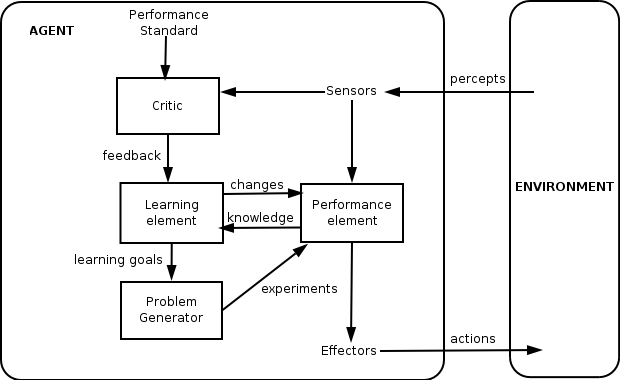
\includegraphics[width=16cm]{resources/schema_agente.png}
    \caption{Schema generale di un agente e dell'ambiente} 
\end{figure}

\subsection{Sistemi multi-agente}
Un sistema multi agente è un sistema computerizzato (inteso anche come sistema distribuito e aperto) composto dalla multipla interazione di differenti agenti intelligenti. Questo tipo di sistemi sono in grado di risolvere problemi che sono difficili o impossibili per un solo ed unico agente o sistema monolitico.
Gli agenti all'interno di questo sistema possono agire in modo indipendente o cooperare tra di loro, inoltre la cooperazione tra questi agenti prevede che essi si scambino dei messaggi tra di loro seguendo dei protocolli o che siano in grado di comunicare rispetto differenti livelli e scopi come: l'obiettivo, l'ambiente, la storia, ecc…
I due aspetti principali dei sistemi multi agente sono:
\begin{itemize}
    \item \textbf{Autonomia}: ovvero la possibilità di un agente di agire liberamente all'interno dell'ambiente rispettando sempre un protocollo e in base all'obiettivo dell'agente.
    \item \textbf{Eterogeneità}: nei sistemi multi agente i protocolli devono specificare il significato dei messaggi in quanto gli agenti interagiscono sulla base dei significati delle loro comunicazioni.
\end{itemize}

All'interno di questo paradigma esiste un altro concetto importante ovvero la coordinazione. Esso è un concetto chiave per lo studio di attività complesse in un sistema dinamico e si occupa di gestire le dipendenze attraverso le varie attività compiute o che devono essere ancora avvenire dagli agenti.
Anche le interazioni possono avvenire in modo differente, ovvero in modo diretto o indiretto.

\begin{figure}[H]
    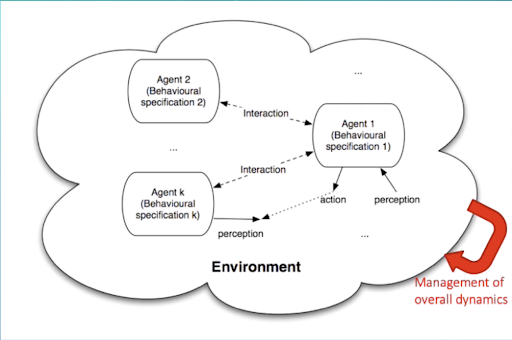
\includegraphics[width=16cm]{resources/agente_modello_riferimento.png}
    \caption{Modello di riferimento di un sistema multi agente all'interno di un ambiente} 
\end{figure}

\subsection{Rete sociale ad agenti}

Una rete sociale \cite{SocialNetworkAnalysis} è una struttura sociale costruita da un gruppo di attori (come ad esempio individui o organizzazioni), una serie di legami diadici (ovvero gruppi che condividono degli interessi comuni e comunicano tra di loro) e altre interazioni sociali tra gli attori. In particolare la prospettiva delle reti sociali fornisce un insieme di metodi per analizzare la struttura di entità sociali e una varietà di conseguenti teorie che possono venire spiegate attraverso la costruzione di modelli osservati all'interno di queste strutture.
Alcuni esempi di questi modelli locali o globali all'interno di queste reti sono l'individuazione di entità influenti oppure l'esame delle dinamiche di evoluzione e adattamente della rete.
L'ambito di ricerca sull'analisi delle reti sociali è certamente interdisciplinare in quanto coinvolge aspetti sociali, psicologici, statistici, informatici, matematici e sicuramente è strettamente legato alla ricerca e allo studio dei complex networks e della network science.

Una rete sociale simulata è appunto una rappresentazione della realtà che presenta determinate caratteristiche. Spesso queste simulazioni però non si relazionano bene con diversi aspetti sociologici delle reali reti sociali in quanto le simulazioni vengono eseguite solamente con reti regolari, casuali, a piccolo mondo e dall'attaccamento preferenziale che non riescono a catturare le sfumature sociologiche degli aspetti sociali. Hamill e Gilbert \cite{SimulatingLargeSocialNetworks} hanno quindi definito delle reti sociali basate sul concetto di agente in modo tale da inserire alcuni aspetti chiave e rilevanti precedentemente non considerati.

Esistono molte reti differenti appartenenti al mondo delle reti sociali, in particolare le reti sociali personali (o ego-centriche) hanno determinate caratteristiche specifiche:
\begin{itemize}
    \item Hanno una dimensione limitata e il loro limite dipende dal tipo di relazione che si sta studiando
    \item Variazione degli individui secondo una distribuzione con coda a destra con un alto grado di connessione per le relazioni molto forti
    \item Altro raggruppamento, ovvero i membri della rete personale di un individuo dovrebbero tendere a conoscersi per riflettere l'omofilia
    \item Cambia nel tempo
\end{itemize}

Ma più in generale un modello di una rete sociale dovrebbe avere:
\begin{itemize}
    \item Una bassa densità di rete nel suo interesse: ovvero solo pochi dei reali e potenziali collegamenti all'interno di una rete dovrebbero esistere
    \item Assortatività positiva del grado di connettività: le persone che hanno una grande rete sociale e conoscono molte altre persone hanno più possibilità di conoscere altre persone che hanno anch'esse un elevato numero di connessioni
    \item Comunità e gruppi di persone saranno molto connesse tra loro stessi, ma avranno poche connessioni con le persone al di fuori della struttura sociale 
    \item È possibile raggiungere le altre persone all'interno della rete con un piccolo numero di passi (concetto di distanza all'interno della rete).
\end{itemize}

All'interno di una rete sociale ad agenti possiamo assistere quindi a differenti e molteplici modellazioni differenti, solitamente in rappresentazioni di questo tipo gli agenti corrispondono agli utenti, alle persone, all'interno della rete e quindi vengono modellati affinchè abbiano delle caratteristiche, delle peculiarità e cerchino di relazionarsi con gli altri agenti attorno a loro ad esempio all'interno di comunità.

Ci sono moltissimi aspetti da considerare nella costruzione di una rete sociale con qualsiasi tecnica di applicazione così come altrettante informazioni e considerazioni possono essere fatte a priori una volta costruito il modello e analizzata la rete simulata.

Definiamo quindi alcuni concetti fondamentali che caratterizzano qualsiasi tipo di rete.

/subsubsection{Comunità}

Una comunità è un insieme di individui che condividono uno stesso ambiente, sia esso fisico e/o tecnologico, formando un gruppo riconoscibile unito da vincoli organizzativi, linguistici, religiosi, economici e da interessi comuni. \cite{Comunita}
Il concetto di comunità è cambiato nel corso della storia umana e si è evoluto al pari passo delle grandi invenzioni tecnologiche come Internet.
All'interno del web troviamo il concetto di Comunità Virtuale \cite{ComunitaVirtuale} diffusa universalmente dal libro The Virtual Community di Hogward Rheingold \cite{VirtualCommunity}. Una comunità virtuale o comunità online è nell'accezione del termine, un insieme di persone interessate ad un determinato argomento, o con un approccio comune alla vita di relazione, che corrispondono tra loro attraverso una rete telematica, come internet, una rete di telefonia, un social network, costruendo una rete sociale con caratteristiche peculiari. È importante sottolineare che all'interno di queste community esiste un concetto di identità proprio all'interno della piattaforma che può o non può corrispondere ad un'identità reale ed un concetto di linguaggio specifico utilizzato all'interno della piattaforma che può portare alla generazione di slang particolari all'interno della stessa.
È infine importante considerare il "senso di comunità" \cite{ComunitaSenso} che unisce i membri all'interno di una stessa comunità che introduce concetti come l'essere membro, l'influenza all'interno del gruppo, l'integrazione e la condivisione di connessioni emotive.
Possiamo quindi evidenziare come la definizione stessa di comunità comporta moltissime accezioni e definizioni differenti a seconda del contesto, della materia o del punto di vista considerato.
All'interno di questo studio siamo principalmente interessati al concetto di comunità virtuale e del senso di comunità esistente all'interno dei social network, in particolare a Twitter.

\subsubsection{Densità della rete}
All'interno di una rete e considerando la social network analysis la densità viene definita come: tutte le possibili "connessioni" esistenti tra i nodi della rete (partecipanti o utenti). È quindi il numero di connessioni che ogni partecipante ha, diviso per il totale delle possibili connessioni che lo stesso utente potrebbe avere \cite{PatternNetworkLearning}

\subsubsection{Lunghezza del cammino (Distanza)}
In matematica e nella teoria dei grafi la distanza tra due vertici in un grafo è espressa come il numero di archi in un percorso più breve (chiamato anche geodetico) che li collega. \cite{GrafoDistanza}
Tra due vertici inoltre possono esistere più percorsi minimi differenti. Se non esiste però un percorso che collega due vertici del grafo, ovvero se appartengono a due componenti non collegate tra di loro, allora convenzionalmente la loro distanza è infinita.
Nel caso di un grafico diretto, la distanza d(u,v) tra due vertici u e v è definita come la lunghezza di un percorso diretto più breve da u a v costituito da archi, purché esista almeno uno di questi percorsi.

\subsubsection{Connessione}
In matematica e informatica, la connettività è uno dei concetti di base della teoria dei grafi ed è una misura importante per la resilienza della rete stessa: 
corrisponde al numero minimo di elementi (nodi o archi) che devono essere rimossi per separare dei nodi in sottografi isolati. \cite{GrafoConnettivita}

In un grafo indiretto $G$, due vertici $u$ e $v$ sono detti collegati se $G$ contiene un percorso $u$ a $v$, altrimenti sono chiamati scollegati. Quando i due vertici sono collegati da un percorso di $lunghezza = 1$, cioè da un singolo bordo, i vertici sono chiamati adiacenti.

Un grafo si dice connesso se ogni coppia di vertici del grafo è connessa, questo comporta che esista un percorso per ogni coppia di vertici, quindi un grafo non diretto che non è collegato viene detto disconnesso. Un grafo non diretto $G$ è quindi scollegato se esistono due vertici in $G$ in modo tale che nessun percorso in $G$ abbia questi vertici come punti finali. Un grafo con un solo vertice è collegato. Un grafico senza archi con due o più vertici è disconnesso.

Infine, un grafo diretto è chiamato debolmente connesso se la sostituzione di tutti i suoi archi diretti con archi non diretti produce un grafo connesso (non diretto). È collegato unilateralmente o unilateralmente (detto anche semiconnesso) se contiene un percorso diretto da $u$ a $v$ o un percorso diretto da v a u per ogni coppia di vertici $u, v$. Mentre è fortemente collegato, o semplicemente forte, se contiene un percorso diretto da $u$ a $v$ e un percorso diretto da $v$ a $u$ per ogni coppia di vertici $u, v$.

\subsubsection{Invarianza di scala}
Un concetto fondamentale all'interno delle reti sociali e anche della rete del World Wide Web è proprio la definizione di rete ad invarianza di scala.
Una rete ad invarianza di scala si definisce tale quando si considera un grafo che ha un numero di connessioni tra vertici ed archi sotto forma di un "esponenziale negativo" e quindi invariante rispetto ai cambiamenti di scala.
Più nel dettaglio il numero di due tipi di nodi, ad esempio uno con 10 connessioni e uno con 15 hanno tra di loro una proporzione che è $\exp(-1 (Nb-Na)) $ dove $Nb$ ed $Na$ sono il numero di nodi del denominatore e numeratore rispettivamente mentre $a$ è un parametro del tipo di rete considerato. Questa legge è detta legge di potenza, di cui $a$ è il parametro \cite{ReteInvarianzaScala}

Empiricamente questa definizione comporta che ci siano degli hub molto densi di nodi e vertici (una comunità o un gruppo di persone) e che quando un nodo deve cercare dei nuovi collegamenti esso lo faccia prima verso un particolare nodo che fa parte di un hub e che ha già molti collegamenti portando il grafo nella sua interessa ad una crescita esponenziale con l'aumentare del numero di collegamenti della rete.

La presenza degli hub e di questo comportamento è alla base della "Teoria del piccolo mondo" anche chiamata dei "6 gradi di separazione" in quanto ogni rete complessa in natura è tale che due qualunque nodi possono essere collegati da un percorso costituito da un numero relativamente piccolo di collegamenti matematicamente determinabile. \cite{TeoriaPiccoloMondo}

\subsection{Misure di valutazione}

Come abbiamo visto precedentemente, nelle reti sociali è importante definire delle misure per spiegare e confrontare un modello o una simulazione rispetto ad un caso reale.
A tal proposito sono state introdotte numerosissime misure e metriche considerabili per valutare la bontà di una rete sociale, esse derivano in grande maggioranza dalla teoria dei grafi in quanto una rete sociale non è nient'altro che un particolare grafo rappresentativo di una realtà o di un sistema.

\subsubsection{Grado e ordine di un grafo}

L'ordine di un grafo \cite{GrafoOrdine} è $|V|$ (il numero dei vertici). La dimensione di un grafo è $|E|$. Il numero di archi incidenti in un vertice $v \in V$ (cioè il numero di archi che si connettono ad esso) prende il nome di grado del vertice $v$, dove un arco che si connette al vertice ad entrambe le estremità (un cappio) è contato due volte.
Si considerano il "grado massimo" e il "grado minimo" di $G$ come, rispettivamente, il grado del vertice di $G$ con il maggior numero di archi incidenti e il grado del vertice di $G$ che ha meno archi incidenti. Quando il grado massimo ed il grado minimo coincidono con un numero $k$, si è in presenza di un grafo k-regolare (o più semplicemente grafo regolare).
Per un arco ${u, v}$, i teorici dei grafi usano solitamente la notazione più sintetica $uv$.
Un grafo $G=(V,\varnothing)$ privo di archi è detto grafo nullo. Un caso estremo di grado nullo è quello del grafo $G=(\varnothing,\varnothing)$, per il quale anche l'insieme dei nodi è vuoto.

Un grafo è definito completo se due qualsiasi dei suoi vertici sono adiacenti (esiste un arco che li connette). La massima cardinalità di un sottografo completo del grafo si chiama densità del grafo.

\subsubsection{Densità di un grafo}

Sia definito il grafo $G=(N,A)$ come coppia dei due insiemi $N={1,2,3,...,n}$ ed $A$ sottinsieme del prodotto cartesiano $N \chi N$. $N$ sarà l'insieme degli n nodi che compongono il suddetto grafo e $A$ l'insieme degli archi.
\begin{itemize}
    \item sia $n$ la cardinalità di $N$ (ovvero il numero dei nodi di un dato)
    \item sia $L$ la cardinalità di $A$ (ovvero il numero degli archi dello stesso grafo)
\end{itemize}
Se le coppie di nodi si considerano ordinate il grafo è detto orientato o digrafo, altrimenti si dice orientato o semplice. Il grafo è detto pesato se ad ogni arco è associato un peso o costo.

La densità di un grafo semplice ($\Delta$) o non orientato è definita come:
\begin{equation}
    \Delta = 2L/n(n-1)
\end{equation}

La densità di un grafo ($\Delta$) orientato è definita come:
\begin{equation}
    \Delta = L/n(n-1)
\end{equation}

Nel caso di grafi pesati ad L occorre sostituire la sommatoria dei pesi di ciascun arco.
La densità di un grafo assume valori compresi tra 0 ed 1 e pertanto si può ricollegare facilmente al concetto di probabilità. La densità di un grafo misura la probabilità che una qualsiasi coppia di nodi sia adiacente, mentre la connessione di un grafo dipende dalla distribuzione degli archi tra i nodi.

Un grafo sconnesso può avere densità maggiore di uno connesso a causa della concentrazione degli archi tra un ristretto numero di nodi.

\subsubsection{Centralità}

Nella teoria dei grafi e nell'analisi delle reti, gli indicatori di centralità \cite{GrafoCentralita} identificano i vertici più importanti all'interno di un grafo. 
Le applicazioni includono l'identificazione della persona o delle persone più influenti in un social network, i nodi infrastrutturali chiave in Internet o nelle reti urbane e i super diffusori di malattie.

Ci sono moltissime misure di centralità che possono essere utilizzate all'interno di un grafo per studiare le caratteristiche e le peculiarità, un'importante misura frequentemente utilizzata è la Betweenness \cite{GrafoBetweenness}

\subsection{Modelli epidemiologici compartimentali}

Con l'avvento del COVID-19 i modelli epidemiologici si sono rivelati fondamentali per comprendere e combattere le situazioni di emergenza che si sono venute a creare nei vari stati.
I primi modelli matematici, anche quelli più utilizzati, che permettono di descrivere i processi di diffusione epidemici arrivano dai lavori di Kermack e McKendrick (1932) e rappresentano ancora oggi uno degli approcci fondamentali per studiare molteplici processi di diffusione dalle malattie, dai virus nel mondo naturale, passando per i virus informatici fino all'analisi di opinioni e contenuti sui social network.

Questi modelli vengono anche chiamati modelli epidemiologici compartimentali \cite{ScienceConnectedAge} perchè alla base del loro ragionamento c'è l'assegnazione di una particolare fetta di popolazione a determinati comportamenti in base a delle caratteristiche epidemiologiche che gli individui hanno. Man mano che l'epidemia evolve e si adatta le persone assumeranno caratteristiche diverse (contrarranno la malattia, guariranno, … ) e quindi cambieranno compartimento allo scorrere del tempo. Lo studio dell'evoluzione delle persone in base alle loro caratteristiche e all'appartenenza ad un compartimento è alla base della costruzione di questi modelli.

Il modello SIR è composto da tre stadi primari che le persone possono assumere rispetto ad una malattia: 
\begin{itemize}
    \item (S) suscettibile, ovvero l'individuo è vulnerabile all'infezione, ma non è ancora stato contagiato
    \item (I) infetto, ovvero l'individuo è stato contagiato e può diffondere la malattia
    \item (R ) rimosso, l'individuo è guarito e ha recuperato lo stato di salute, oppure è deceduto
\end{itemize}

\begin{figure}[H]
    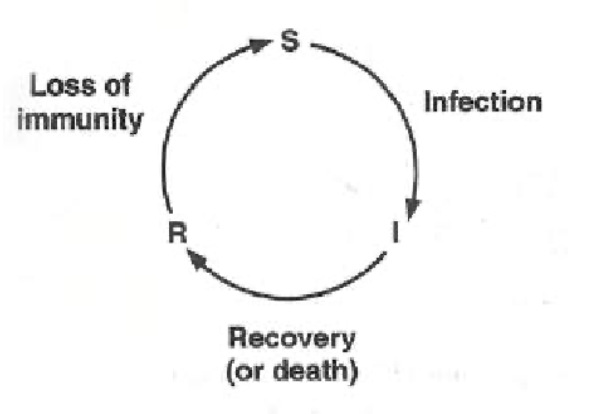
\includegraphics[width=16cm]{resources/sir_circle.png}
    \caption{Schema di riferimento per il modello SIR} 
\end{figure}

Oltre alla caratterizzazione delle persone esistenti all'interno di uno scenario, il modello SIR considera una distribuzione di probabilità da parte delle persone suscettibili di essere infettate che dipende strettamente dal grado di infettività di una malattia. Nei primi lavori in questo campo per semplificare le studio delle dinamiche, lo studio della probabilità di diffusione venne influenzata dalla numerosità delle popolazioni di infetti e suscettibili e dalla variazione dei parametri di controllo: il grado di infettività e il tasso di recupero.

In tale modello l'infezione segue un andamento di crescita logistica, quando l'epidemia inizia si ha una piccola porzione di elementi infetti. Al passo successivo spesso si evidenzia una fase di lenta crescita che corrisponde anche al momento migliore per bloccare la diffusione della malattia nonostante la difficoltà nella distinzione dell'epidemia e da casi sparsi non correlati tra di loro. Se la diffusione procede nel tempo si entra nella fase esplosiva della crescita logistica e diventa molto difficile riuscire a fermarla. L'ultima fase è quella di esaurimento in quanto la popolazione dei suscettibili diventa troppo piccola affinchè l'epidemia continui a diffondersi.

\begin{figure}[H]
    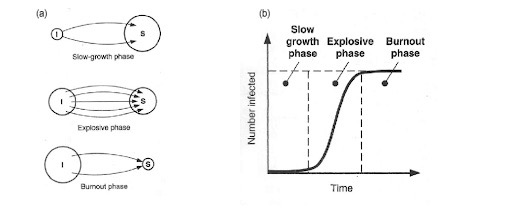
\includegraphics[width=16cm]{resources/tasso_sir_2.jpeg}
    \caption{Tassi dei nuovi infetti in dipendenza dalel dimensioni delle popolazioni di suscettibili ed infetti in cui i tassi di crescita sono massimizzati per la fase esplosiva della crescita logistica (a). In (b) il diagramma della crescita logistica con il suo caratteristico andamento della curva ad "S" che mostra una fase di bassa crescita (slow-growth), una fase esplosiva (explosive phase) e una fase di esaurmento (burnout phase)} 
\end{figure}

Il modello a crescita logistica segue quindi nell'arco delle tre fasi un andamento caratterizzato dalla forma ad "S" e la sua diffusione dipende soprattutto dalla capacità di infettare gli individui. La contagiosità (chiamata anche tasso di crescita) è regolata all'interno del modello dal tasso di riproduzione, ovvero il numero medio di nuovi infetti generati da ogni singolo individuo malato.
La condizione del tasso di riproduzione affinché la malattia entri nella fase esplosiva è che il tasso sia superiore a 1, qualora fosse inferiore gli infetti verrebbero rimossi più velocemente rispetto al numero dei nuovi infetti. Il tasso di riproduzione rappresenta quindi il concetto di soglia critica dell'epidemia.
Questa prima modellazione e spiegazione dei modelli SIR si basavano su reti semplici e casuali tuttavia nel mondo della scienza delle reti troviamo moltissime tipologie di reti differenti che modellano particolari condizioni i cui risultati sono incerti e interessanti da analizzare, ecco perché i modelli SIR e derivati hanno ancora oggi una grande applicazione in quanto consentono di adattarsi bene a moltissime reti differenti pur mantenendo un'elevata capacità espressiva facilmente calcolabile.
È importante considerare che nel corso del tempo ci sono state diverse evoluzioni del modello per costruire nuovi compartimenti utili a studiare differenti punti di vista di una situazione epidemiologica (come ad esempio il fatto che una persona non riesce mai a guarire del tutto e continua ad essere contagiosa anche a distanza di molto tempo) o per modellare un determinato problema come ad esempio SEIR (Suscettibile Esposto Infetto Rimosso), SEIS (le persone rimangono sempre nello stato di Suscettibilità anche dopo l'infezione e quindi nel tempo) e molte altre differenti variazioni e modellazioni.

\section{Stato dell'arte}

\section{SOIL}

\section{Soluzione proposta}

\subsection{Grafo}

\subsection{Opinion Leader}

\subsection{Bot}

\subsection{Simulazioni}

\subsection{Configurazione di SOIL}

\subsubsection{File Python}

\subsubsection{File YML}

\subsection{Web app}

\subsubsection{Uso di streamlit}

\section{Risultati ottenuti}

<<<<<<< HEAD
\subsection{Random}


\subsection{Betweenness e In-Degree}

\subsection{Eigenvector}

\section{Conclusioni}

Per quanto riguarda la fase di validazione non è stata possibile attuarla. A causa delle forti limitazioni nell'uso di Twitter dovute ad un restringimento delle policy di sicurezza e di accesso non siamo riusciti a validare il modello su casi reali. Le informazioni utilizzate all'interno delle analisi e la topologia della rete sono state ottenute effettuando uno scraping limitato proprio sui dati di twitter. Per la validazione del modello occorrerebbe avere a disposizione più dati e informazioni in modo da migliorare la fase di validazione e valutazione rispetto, ad esempio, a delle situazioni realistiche di diffusione e contaminazione di notizie che si sono verificate nel tempo.


\section{Sviluppi futuri}

Dopo aver costruito il simulatore e aver portato i risultati e le considerazioni derivanti dal processo di sperimentazione definiamo quelli che saranno gli sviluppi futuri del progetto.

A tal proposito vengono proposte due aree di miglioramento e di sviluppo: la prima legata all'applicazione e alla parte tecnica, mentre la seconda dedicata alla parte modellistica e progettuale.

Per quanto riguarda l'area applicativa:
\begin{itemize}
    \item \textbf{Miglioramento della UX}: rendere migliorabile la user experience dell'applicazione web in modo da renderla facilmente fruibile e distribuibile ad una più larga utenza
    \item \textbf{Miglioramento delle performance}:  è necessario incrementare le performance per quanto riguarda la velocità di computazione e di calcolo delle statistiche, modelli e grafici.
    \item \textbf{Deploy dell'applicazione}: rilascio dell'applicazione in un ambiente di produzione con sufficienti requisiti hardware per consentire e favorire numerosi simulazioni anche con più dimensionalità riducendo il limite infrastrutturale avuto durante la prima fase realizzativa
    \item \textbf{Aggiornamento del codice e della repository}: favorendo un approccio più OpenSource in modo che la soluzione sia più facilmente mantenibile e aggiornabile
    \item \textbf{Accesso ad hardware più performance}: in fase di valutazione per il lancio di simulazioni massive.
\end{itemize}

Per quanto riguarda invece la parte modellistica:

\begin{itemize}
    \item \textbf{Arricchire la modellazione degli utenti}: Cercare di distinguere ulteriormente gli utenti in modo da definire delle categorie di utenza all'interno di una rete sociale in modo che siano configurabili e conseguentemente arricchire le categorie con attributi unici per utente come il genere, informazioni personali, … oltre a rendere ancora più specifico l'inserimento dei bot all'interno della rete in modo tale da definire ad esempio la frequenza di pubblicazione, i tipi di pubblicazioni o altro… Allo stesso tempo anche gli Opinion Leader e le conseguenti sottoreti di cui fanno parte possono essere modellati in modo da rispecchiare ancora di più un caso reale.
    \item \textbf{Ottenere riscontro da dati reali}: A causa delle forti limitazioni nell'uso dei social network dovuto ad un restringimento dello politiche di sicurezza e privacy abbiamo riscontrato moltissime difficoltà nella valutazione e misurazione delle performance rispetto ad un caso reale. Avere a disposizione dei dati reali di alcune situazioni verificatesi in passato o ad una configurazione della rete più realistica ci consentirebbe di potenziare e migliorare la fase di valutazione e validazione dei risultati rispetto al nostro modello implementato.
    \item \textbf{Caratterizzazione dei contenuti}: All'interno del modello e del sistema multi-agente non abbiamo effettuato una distinzione del tipo di contenuti diffusi, la possibilità di caratterizzare i contenuti ad esempio con dei topics consentirebbe di definire e modellare comportamenti più simili alla realtà andando a studiare anche a livello contenutistico la diffusione dei post all'interno della rete.
    \item \textbf{Informazioni di contesto}: Rispetto ai contenuti e agli utenti, anche alcune informazioni di contesto potrebbero migliorare e rendere il sistema più simile alla realtà. Queste informazioni potrebbero essere ad esempio: tempi di pubblicazione delle news (a livello orario), informazioni geospaziali come luoghi o parti del mondo, tempi e facilità di accesso alla piattaforma dove gli utenti interagiscono, ecc...
    \item \textbf{Test con nuovi algoritmi}: implementare ulteriori algoritmi epidemiologici per la diffusione di notizie per identificare il migliore modello da realizzare all'interno del sistema.
    \item \textbf{Simulatore personalizzato}: costruzione di un simulatore personalizzato per questo specifico task in modo da potenziare e rendere più specifico l'impiego di un sistema multi agente in questo determinato contesto, ma allo stesso tempo più personalizzabile e ottimizzato
\end{itemize}

\bibliographystyle{plainurl}
\bibliography{bibliography}



\end{document}
